\chapter{Modelo de lattice Boltzmann}

\graphicspath{{figs/cap2/}}
\label{cap2}

\section{LBM Multifásicos}

En éste capítulo se presentara cuál es el modelo de LB para la resolución de problemas de transferencia de calor con flujos multifásicos y cambio de fase.

Generalmente es difícil resolver las ecuaciones de la mecánica de los fluidos. Las soluciones analíticas de los problemas que pueden ser halladas son escasas, como el caso de flujos \textit{Couette} o \textit{Poisueuille}. Problemas que contengan una geometría más compleja u otras condiciones de contorno; poseen una gran dificultad para encontrar la solución de las ecuaciones de la mecánica de fluidos, si es que el problema la posee. Debido a ello las soluciónes se obtienen numéricamente \cite{kruger2017lattice}(Sec 3.1). Es de importancia el desarrollo de métodos numéricos que resuelvan los problemas de forma paralela para así reducir el tiempo de cálculo.

Los problemas que se plantean resolver en el presente trabajo son de transferencia de calor en flujos multifásicos con cambio de fase, la escala de fluido que se decide adoptar es la mesoscópica. Considerando la escala y siendo un problema multifásico, se opta por resolver numéricamente mediante LBM. 


Los mayoría de los modelos para resolver los flujos multifásicos son tres clasificados en cuatro categorias generales : \textit{color gradient}, \textit{Shan Chen model} o \textit{pseudopotential}, \textit{Free-energy} y  \textit{phase-field}. 


\begin{itemize}
	
	\item \textit{Color gradient} fue el primer modelo de LBME para flujos multifásicos siendo desarrollado por Gunstensen \cite{gunstensen1991lattice}. Las fases y las interacciones entre las partículas son denotadas mediante diferentes colores. Por medio del modelado local del gradiente de color que se encuentra asociado a la diferencia de las densidades de las dos fases, se conoce como es la segregación y separación de las fases.
	
	\item \textit{Shan Chen model} o \textit{pseudopotential} surge de representar la fenomenología de \textit{color gradient} por medio de una redistribución de las particulas del fluido. La fuerza de interacción proviene de la diferencia entre las fuerzas promedio del modelo molecular  entre ambos lados de la interfaz. Shan and Chen \cite{shan1993lattice} presentaron un modelo de LBE (referenciado como modelo SC) que podría representar la interacción entre partículas fluidas de forma más precisa y directa introduciendo un pseudo potencial. 
	
	\item \textit{Free-energy} es un tipo de modelo alternativo de LBE desarrollado por Swift \cite{swift1995lattice} para modelos multifásicos/multicomponentes basado en la teoría de energía libre (\textit{free-energy}). La idea básica del nuevo método es realizar una función de distribución de equilibrio basada en funciones de energía libre, en las cuales se incorpora el tensor de presión termodinámico.\cite{guo2013lattice}(sec 7).
	
	\item \textit{Phase-field} utiliza en su modelo un parámetro gobernado por una ecuación de tipo convección-difusión para realizar un seguimiento de la interfaz. Presenta una gran estabilidad numérica y precisión para problemas con grandes relaciones de densidad y viscosidad \cite{wang2019brief}.
	
	\iffalse
	Debido a que la fenomenología representada en los modelos de LBE de color y pseudo potenciales son la misma. \textbf{se corta la oracion}
	\fi
	
\end{itemize}





\section{Modelo pseudopotencial}

El modelo pseudopotencial es el adoptado en el presente trabajo para abordar los problemas descriptos en el Cap. (\ref{cap4}) por lo cual se detalla en ésta sección. Este modelo multifásico tiene la particularidad de que la frontera entre las fases no es resuelta con exactitud. Dicha interfaz es representada de forma difusa con un cierto tamaño en la grilla, siendo una importante ventaja para el cálculo puesto que la interfaz no debe ser reconstruida.\cite{parrill2019reviews}.


La obtención de la ecuación de lattice Boltzmann (LBE) a través de la ecuación de Boltzmann se encuentra descripta en \cite{kruger2017lattice} (Sec 3.4 y 3.5 ). Primero se explica la discretización en el espacio de velocidades, en el segundo la del espacio físico, temporal e integración de las características.


El problema físico a resolver cuenta con una región, la cuál se le realizará un mallado para discretizar el espacio. El nodo i - ésimo de la malla posee las coordenadas ${\bar{X}}_{i} = (x,y,z)$, a su vez densidad $\rho_{i}$ y temperatura $T_{i}$. La velocidad en el nodo tiene las componentes ${\bar{U}}_{i} = ({U}_{ix},{U}_{iy},{U}_{iz})$. El espacio de velocidades indica como es la propagación de las propiedades en la grilla. Dicha velocidad de grilla $\mathbf{e}_{i}$ posee $\alpha$ componentes donde $\alpha = q $. 

En el presente trabajo el LBM es $D2Q9$, el esquema de velocidades de grilla para el nodo i-ésimo del D2Q9 es el presentado en la Figura \ref{fig:D1Q3_D2Q9}. La Ec. (\ref{eq:velgrilla}) detalla los valores de velocidad adoptados. 

Cada nodo de la grilla contará con una distribución $f_{i}$, asociada al espacio de poblaciones. En el caso más simple se cuenta con una distribución y esa asociada a la densidad. La distribución $f_{i}$ posee $\alpha$ componentes. Mediante ésta funcion de distribución, pueden recuperarse variables macroscópicas del problema, como ser : $\rho$ , $U$,$T$.

En éste modelo la distribución $f$ se calcula a través de las fuerzas de interacción que poseen las partículas de cada nodo. Por lo que se debe proporcionar un potencial que describa a las fuerzas de interacción, dicho potencial estará dado por una Ecuación de estado (\textit{Equation of state} o EOS).

Es de importancia la elección de la EOS a utilizar, puesto que según ella se recupera el tensor de presión, las variables $\rho$ , $U$ , $T$ ; a una dada presión y temperatura las densidades de coexistencia de líquido y gas, como el calor latenten entre otras propiedades intrínsecas del fluido.

\section{Ecuación de estado y fluido de Van der Waals}

Al ser multifásicos los problemas a desarrollar, es de importancia conocer las leyes que gobiernan las fases de los fluidos. La ley de gases ideales \ref{eq:gas_ideal} es una EOS , cabe destacar que la mayor supusición es que las partículas del gas son puntuales. Donde \textit{p} es la presión (atm), V es el volúmen (L), \textit{n} número de moles, R constante universal de los gases y \textit{T} temperatura. La Ley caracteriza el comportamiento para gases de baja densidad.

\begin{align}
p V = n R T
\label{eq:gas_ideal}
\end{align}

La EOS de Van der Waals (VdW) \ref{eq:VdW_P} fue propuesta para caracterizar el comportamiento de los gases reales, siendo $V_m = \frac{V}{n}$ el volúmen molar. Las constantes \textit{a} y \textit{b} son características de cada fluido.

\begin{align}
p = \frac{R T}{V_m - B} - A {(\frac{1}{V_m})}^2
\label{eq:VdW_P}
\end{align}

El parámetro \textit{A}  ($\frac{atm L^2}{mol^2}$) caracterizan la interacción que poseen las moléculas del gas entre sí, y \textit{B} ($\frac{L}{mol}$) da una idea del volumen molar mínimo que posee una partícula del fluído (éste parámetro define a la partícula del gas con un dado volúmen en vez de ser puntual como en la Ley de gases ideales).

La EOS de VdW es utilizada en el presente trabajo para modelar el potencial del modelo LBM \textit{pseudopotential} de interacción entre las partículas.


\section{Modelo pseudopotencial de dos ecuaciones con operador MRT}
\label{sec:LBM_2_ec_MRT}

En ésta sección se describirá cuál es el LBM que se utilizará para resolver los problemas descriptos en el Cap. \ref{cap4}. La denominación del tipo de operador, \textit{multiple relaxation times} o MRT, proviene por los parámetros que se deben ajustar y proponer para que el modelo concuerde con los valores esperados.

Se deben resolver dos ecuaciones, la primera es la hidrodinámica que representa a la conservación de masa y momento; la segunda a la de energía, descriptas en \colorbox{green}{citar paper con la ec de energia}.


\subsection{Ecuación hidrodinámica}

Por medio de la función de distribución Ec. \ref{eq:fieldmom} \cite{li2013lattice} se realiza la resolución de la ecuación hidrodinámica,


\begin{equation}
    \mathbf{f}(\mathbf{x} + \mathbf{e} \> \delta_{t} , t + \delta_{t}) = \mathbf{M}^{-1} \left[ \mathbf{m} - \mathbf{\Lambda}(\mathbf{m} - \mathbf{m}^{(eq)}) + \delta_{t} \left( \mathbf{I} - 0,5 \mathbf{\Lambda} \right) \mathbf{\bar{S}}  \right]_{(\mathbf{x},t)} 
    \label{eq:fieldmom}
\end{equation}\\
donde $\mathbf{x}$ es la posición espacial, \textit{t} el tiempo, $\delta_{t}$ el paso de tiempo , \textit{\textbf{e}} la velocidad de grilla en sus direcciones $\alpha$ y $\textit{f}$ es la distribución de densidad en el espacio de poblaciones. La notación utilizada implica que la componente $\alpha$-ésima del miembro izquiero de la Ec. (\ref{eq:fieldmom}) esté dado por $f_{\alpha}(x + e_{\alpha} \delta_{t}  , t + \delta_{t} )$. El miembro derecho de la Ec. (\ref{eq:fieldmom}) corresponde a la etapa de post-colisión definida en el espacio de momentos, donde \textbf{I} es el tensor identidad, \textbf{M} una matriz de transformación ortogonal, $\mathbf{m} = \mathbf{M} \cdot \mathbf{f}$ , $\mathbf{m}_{eq} = \mathbf{M} \cdot \mathbf{f}_{eq}$ , $\mathbf{\bar{S}} = \mathbf{M} \mathbf{S}$ el término de fuente y $ \Lambda$ es una matriz diagonal.

Para el modelo de grilla D2Q9 utilizado en el presente trabajo $\mathbf{m}_{eq}$ y $ \Lambda$ están dados por Ec. \ref{eq:m} y \ref{eq:lambda} respectivamente.

\begin{align}
m_{eq} =  \rho  \left( 1, - 2 + 3 {|u|}^{2} , 1 - 3{|u|}^{2} , u_{x} , - u_{x} , u_{y} , - u_{y} , {u_{x}}^{2} - {u_{y}}^{2} , u_{x} u_{y} \right) 
\label{eq:m}
\end{align}

    
\begin{align}
    \mathbf{\Lambda}  = diag ( {\tau_{\rho }}^{-1},{\tau_{e}}^{-1},{\tau_{\zeta }}^{-1},{\tau_{j}}^{-1},{\tau_{q}}^{-1},{\tau_{j}}^{-1},{\tau_{q}}^{-1},{\tau_{\nu }}^{-1},{\tau_{\nu}}^{-1}) 
    \label{eq:lambda}
\end{align}


La densidad macroscópica es obtenida mediante la Ec. (\ref{eq:rho}).

\begin{equation}
        \rho = \sum_{\alpha} f_{\alpha}
        \label{eq:rho}
\end{equation}

Por medio de la Ec. (\ref{eq:U}) se obtiene la velocidad.

\begin{equation}
    \rho \> \mathbf{u} = \sum_{\alpha} {\mathbf{e}}_{\alpha} \> f_{\alpha} + 0,5 \> {\delta}{t} \> \mathbf{F}
    \label{eq:U}
\end{equation}

Para el modelo D2Q9 la fuerza total $\mathbf{F}$ posee sólo dos componentes $F_{x} , F_{y}$. Donde $ {\mathbf{F}} = {\mathbf{F}}_{b} + {\mathbf{F}}_{int} $, siendo ${\mathbf{F}}_{b}$ la fuerza volumétrica y ${\mathbf{F}}_{int}$ la fuerza de interacción que hay en el sistema dadas por Ec.(\ref{eq:Fb}) y (\ref{eq:fint}) respectivamente.

\begin{equation}
	{\mathbf{F}}_{b} = \rho \> \mathbf{g}
	\label{eq:Fb}
\end{equation}


\begin{equation}
{\mathbf{F}}_{int} = - G \> \psi(\mathbf{x}) \sum_{\alpha=1}^{N} w({|{\mathbf{e}}_{\alpha}|}^{2}) \> \psi (\mathbf{x} + {\mathbf{e}}_{\alpha} \> \delta_{t}) \> {\mathbf{e}}_{\alpha} 
\label{eq:fint}
\end{equation}

Donde G corresponde a la intensidad de interacción, $w({|{\mathbf{e}}_{\alpha}|}^{2})$ son los pesos correspondientes a una grilla D2Q9 y $\psi$ es el potencial :

\begin{equation} 
    \psi(\rho) = \sqrt{\frac{2 (p_{EOS} - \rho \> {c_{s}}^{2})}{G {c}^{2}}}
    \label{eq:psi}
\end{equation}

Donde $c_{s}$ es la velocidad del sonido en el medio, la EOS adoptada en el presente trabajo es la de VdW :

\begin{equation}
    p_{EOS} = \frac{\rho R T}{1- \rho \> b} - a {\rho}^{2}
    \label{eq:rho_eos}
\end{equation}

donde \textit{a} y \textit{b} son parámetros que determinan los valores críticos de temperatura, presión y densidad. Finalmente, la fuerza de interacción se incorpora en la etapa de colisión mediante un término de fuente apropiado:


\begin{equation}
    \bar{S} = 
    \left[ \begin{array}{c} 
        0\\
        6 \mathbf{u}\cdot \mathbf{F} + \frac{12 \sigma {|{\mathbf{F}_{int}|}}^{2} }{{\psi}^{2} \delta_{t} (\tau_{e} - 0,5)}\\
        6 \mathbf{u}\cdot \mathbf{F} - \frac{12 \sigma {|{\mathbf{F}_{int}|}}^{2} }{{\psi}^{2} \delta_{t} (\tau_{\zeta } - 0,5)}\\
        F_{x}\\
        -F_{x}\\
        F_{y}\\
        -F_{y}\\
        2(u_{x} F_{x} - u_{y} F_{y} )\\
        (u_{x} F_{x} + u_{y} F_{y} )\\              
    \end{array}
    \right]    
    \label{eq:termino_fuente_s}
\end{equation}
\\
donde $\sigma$ es un parámetro libre del modelo MRT, al igual que $\Lambda$ , el cual se utiliza para ajustar las diferencias de fases obtenidas de la EOS y de la simulación realizada.

Se puede recuperar la ecuación de Navier - Stokes utilizando Ec. [\ref{eq:rho} - \ref{eq:termino_fuente_s} ] mediante el análisas de Chapman-Enskog limitado para un número de Mach bajo \cite{li2013lattice}. Siendo las ecuaciones recuperadas \cite{fogliatto2019simulation} \cite{li2013lattice}:

\begin{equation}
	\frac{\partial \rho }{\partial t}  + \nabla \cdot \left( \rho \mathbf{u} \right) = 0
\end{equation}
\begin{equation}
	\frac{\partial \left( \rho \mathbf{u}\right)}{\partial t} + \nabla \cdot \left( \rho \mathbf{u} \mathbf{u}\right) = - \nabla \left( \rho {c_{s}}^{2} \mathbf{I} \right) + \nabla \mathbf{\Pi} + \mathbf{F} - 2 G^{2} c^{4} \sigma \nabla \left( {|\nabla \psi	|}^{2} I	\right) + O (\partial^{5})
\end{equation}
\begin{equation}
\mathbf{F} = - G c^{2} \left[	\psi \nabla \psi + \frac{1}{6} c^{2} \psi \nabla \left( \nabla^{2} \psi\right) + ...\right] + \mathbf{F}_{b} = \mathbf{F}_{int} + \mathbf{F}_{b}
\end{equation}
\\
Donde $\mathbf{\Pi}$ es el tensor de viscosidad dado por :

\begin{equation}
	\mathbf{\Pi} = \rho \nu \left[	\nabla \mathbf{u} + {\left(\nabla \mathbf{u}\right)}^{T}\right] + \rho \left(\ \xi - \nu \right) \left( \nabla \mathbf{u}\right) \mathbf{I}
\end{equation}
\\
siendo $\quad\nu = {c_{s}}^{2} (\tau_{\nu}- 0,5) \delta_{t}\quad$ la viscosidad cinemática y $\quad\xi = {c_{s}}^{2} (\tau_{\nu}- 0,5) \delta_{t}\quad$ la viscosidad volumétrica.



\subsection{Ecuación energía}

Para tener en cuenta la transferencia de calor en el modelo, es necesario adicionar otra ecuación de LB acoplandola con la primera\cite{li2013lattice}. Para nuestro caso, se utiliza la distribución de poblagicones \textit{g} en la Ec. (\ref{eq:fieldenergy}), la cuál también posee un operador de colisión MRT. Donde $\mathbf{n} = \mathbf{M} \mathbf{g}$ es una distribución de momentos y $\hat{\Gamma}$ es una fuente en el espacio de momentos.


\begin{equation}
    \mathbf{g}(\mathbf{x} + \mathbf{e} \delta_{t} ,t + \delta_{t}) = \mathbf{M}^{-1} \left[ \mathbf{n} - \mathbf{Q}(\mathbf{n} - \mathbf{n}^{(eq)}) + \delta_{t} \left( I - 0,5 Q \right) \hat{\Gamma}  \right]_{(\mathbf{x},t)}
    \label{eq:fieldenergy}
\end{equation}

En éste caso los parámetros libres del modelo MRT vienen dados en parte por la matriz de coeficientes de relajación \textbf{Q}, siendo compuesta por la diagonal que se indica en Ec.(\ref{eq:Q_matriz}) y además por los elementos no nulos $Q_{3,4}$ y $ Q_{5,6}$ que se indican en Ec. (\ref{eq:Q_34}) y (\ref{eq_Q_56})  respectivamente.

\begin{equation}
    \textit{diag} (Q) = {( q_{0} , q_{1} , q_{2} , q_{3} , q_{4} , q_{5} , q_{6} , q_{7} , q_{8} )}^{T}
    \label{eq:Q_matriz}
\end{equation}
\begin{equation}
    Q_{3,4} = q_{4} \left( \frac{q_{3}}{2} - 1 \right)
    \label{eq:Q_34}
\end{equation}
\begin{equation}
    Q_{5,6} = q_{6} \left( \frac{q_{5}}{2} - 1 \right)
    \label{eq_Q_56}
\end{equation}

La distribución de equilibrio $\mathbf{n}_{eq}$ se encuentra definida en Ec.(\ref{eq:n_eq}), siendo $\alpha_{1}$ y $\alpha_{2}$ parámetros libres del modelo MRT.

\begin{equation}
    {\mathbf{n}}_{eq} = T { \left( 1, \alpha_{1}, \alpha_{2}, u_{x}, -u_{x}, u_{y}, -u_{y}, 0, 0 \right) }^{T}
    \label{eq:n_eq}
\end{equation}

La temperatura macroscópica \textit{T} puede recuperarse mediante:

\begin{equation}
T = \sum_{\alpha} g_{\alpha} + \frac{1}{2} \delta_{t} {\hat{\Gamma}}_{0}
\end{equation}



Siendo el término fuente :


\begin{equation}
    \hat{\Gamma} = {( s, 0, 0, 0, 0, 0, 0, 0, 0 )}^{T}
\end{equation}

con 

\begin{equation}
    s = \frac{\chi}{\rho} \nabla T \cdot \nabla \rho + T \left[ 1 - \frac{1}{\rho c_{\nu}} {\left( \frac{\partial p_{EOS}}{\partial T} \right)}_{\rho} \right] \nabla \cdot \mathbf{u}
    \label{eq:s_chica}
\end{equation}

La recuperación de la ecuación del calor por medio de Ec. [\ref{eq:fieldenergy} - \ref{eq:s_chica} ] resulta \cite{markus2011simulation}:

\begin{equation}
    \frac{\partial T}{\partial t} + \nabla \cdot ( \mathbf{u} T ) = \chi \> {\nabla }^{2} T + s
\end{equation}

Donde $\chi$ es la difusividad térmica, considerándose constante por simplicidad, obteniéndose mediante Ec. (\ref{eq:chi}). La difusividad térmica queda determinada por los coeficientes de relajación $\mathbf{Q}$ y los parámetros libres $\alpha_{1}$ y $\alpha_{2}$ de ${\textbf{n}}_{eq}$.

\begin{equation}
    \chi = \delta_{t} \left( \frac{1}{q_{3}} - \frac{1}{2} \right) \left( \frac{ 4 + 3 \alpha_{1} + 2 \alpha_{2}}{6} \right)
    \label{eq:chi}
\end{equation}

\subsection{Condiciones de contorno}

Cuando se implementa la colisión en los nodos que se encuentran en la frontera de la región a resolver, no se poseen todos los valores de la función de distribución de poblaciones $\mathbf{f}$ y $\mathbf{g}$, por lo que es necesario determinar cómo se obtienen los mismos. 

Los problemas que se desarrollarán en el Cap. \ref{cap4} tienen una región rectangular o cuadrada, con la particularidad que sus  condiciones de contorno en los bordes es periódica, ya sea en el eje \textit{X}, \textit{Y} o en ambos. Por lo que no existe la dificultad de fijar los valores de $\mathbf{f}$ y $\mathbf{g}$ en nodos que se encuentran en los vértices de la región. Siendo los casos a desarrollar  el de los nodos que se encuentran en las aristas del cuadrado o rectángulo. Las cuatro (4) aristas de la región se resuelven de forma idéntica por lo que sólo se  desarrollará una.

La Figura (\ref{fig:CC_hidro}) ilustra las direcciones de las componentes de $\mathbf{f}$ y $\mathbf{g}$ para un nodo que se encuentra en la frontera. La disposición observada es la que se evaluará para las condiciones de contorno hidrodinámica y de energía.  

\begin{figure}[h!]
	\centering
	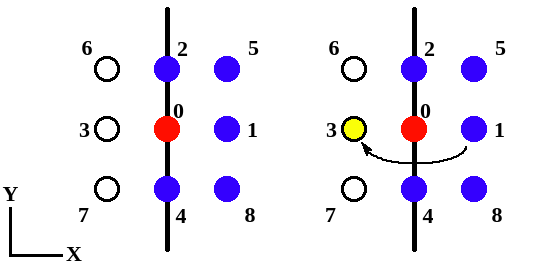
\includegraphics[width=0.85\textwidth]{figs/cap2/CC_hidrodinamica.png}
	\caption{Bloques de threads organizados en una grilla de bloques \cite{rinaldi2011modelos}.}
	\label{fig:CC_hidro}
\end{figure}

Por convención las direcciones que se conocen los valores de las funciones de distribución pertenecen al conjunto A y las que no se conocen al conjunto B. Por lo que $ 0, 1, 2, 4, 5, 8 \in A$ y $ 3, 6, 7 \in B$ 


\subsubsection{Condición hidrodinámica}

El desarrollo de Zou \cite{zou1997pressure} es el utilizado para la ecuación hidrodinámica. Primeramente el método \textit{bounceback} es aplicado a la dirección \textit{3}, resultando $f_{3} = f_{1}$ como se observa en la Figura \ref{fig:CC_hidro}. Luego se analizan las Ec. (\ref{eq:rho}) y (\ref{eq:U}) que son puestas de la siguiente forma:

\begin{equation}
	\begin{array}{c}
	f_{3} + f_{6} + f_{7} = \rho - \left( f_{0} + f_{1} + f_{2} + f_{4} + f_{5} + f_{8}	 \right)\\
	f_{6} - f_{7} = \rho u_{x} - \left( f_{1} - f_{3} - f_{7} + f_{8} 	 \right)\\
	f_{3} + f_{6} + f_{7} = \rho u_{y} + \left( f_{1} + f_{5} + f_{8} \right)
	\end{array}
\end{equation}

Para finalizar se aplican las condiciones de no deslizamiento, para éste caso $\> u_{y} = 0\quad$ y $\quad\mu \frac{\partial u}{\partial x} = \tau_{wall}\quad$, siendo $\tau_{wall}$ el esfuerzo de corte realizado en la arista analizada. Se obtenienen las siguientes condiciones de contorno a la distribución de poblaciones $\mathbf{f}$:

\begin{equation}
\begin{array}{c}
f_{i3} = f_{i1}\\
f_{i7} = f_{i5} - 0,5 (f_{i4} - f_{i2}) - 0,25 (F_{ix} + F_{iy})\\
f_{i6} = f_{i8} + 0,5 (f_{i4} - f_{i2}) - 0,25 (F_{ix} + F_{iy})\\
\end{array}
\end{equation}

donde el índice \textit{i} indica que es el nodo \textit{i}-ésimo que de la arista y $F_{ix}$, $F_{iy}$ es la fuerza del nodo. 


\subsubsection{Condición de energía}

La condición de contorno a realizar en la ecuación de energía, es mantener una temperatura fija en una de las aristas o en secciones de la misma. Por lo cual se utiliza el desarrollo de Inamuro \cite{inamuro2002lattice}.

Primeramente se calcula el valor de la distribución de equilibrio del nodo $i$-ésimo $\mathbf{g}_{eq\>i}$ utilizando Ec. (\ref{eq:n_eq}) y $\mathbf{M}$ de la forma $\mathbf{g_{eq}} = \mathbf{M}^{-1} \mathbf{n_{eq}}$. Se prosigue a calcular el parámetro $\beta$:

\begin{equation}
\beta = \frac{T_{cc} - \sum_{A} g_{A}}{\sum_{B} g_{B}}
\label{eq:beta}
\end{equation}

donde $T_{cc}$ es la temperatura fijada como condición de contorno, $g_{A}$ adopta los valores conocidos de las direcciones pertenecientes al cpnjunto A ($0, 1, 2, 4, 5, 8 $), mientras que $g_{B}$ adopta los valores de la dirección de $\mathbf{g_{eq}}$ calculada recientemente para las direcciones de B ($3, 6, 7$).

Por último en las direcciones del conjunto B, el valor de $g$ resulta:

\begin{align}
	g_{B} = \beta \> g_{eq \> B} 
\end{align}

A modo de ejemplo se detalla el valor que adoptará la dirección \textbf{3}:

\begin{equation}
	g_{3} = \frac{T_{cc} - \overbrace{\left( g_{0} + g_{1} +g_{2} + g_{4} + g_{5} + g_{8} \right)}^{\sum_{A} g_{A}} }{\underbrace{\left( g_{eq\>3} + g_{eq\>6} + g_{eq\>7} \right)}_{\sum_{B} g_{B} }} \quad g_{eq\>3}
\end{equation}


%%% Local Variables: 
%%% mode: latex
%%% TeX-master: "template"
%%% End: 
